% EE2000 Mid-Term Project Report -- Fall 2026, IIT Hyderabad
% Topic: Real-Time EEG Seizure Detection on FPGA (DWT + Linear SVM)
% Template: IEEE/CVF (cvpr.sty review format)
% Note: All content added since Preliminary Project Report is strictly marked in blue text.

\documentclass[10pt,twocolumn,letterpaper]{article}

\usepackage[review]{cvpr} 
\usepackage{graphicx}
\graphicspath{{../results/}{results/}}
\usepackage{amsmath}
\usepackage{amssymb}
\usepackage{booktabs}
\usepackage{tabularx}
\usepackage{tikz}
\usetikzlibrary{arrows.meta,positioning,fit,backgrounds}
\usepackage[dvipsnames]{xcolor}

\usepackage[pagebackref,breaklinks,colorlinks,allcolors=cvprblue]{hyperref}
\def\paperID{15}
\def\confName{EE2000}
\def\confYear{2026}

\title{Real-Time EEG Seizure Detection Using Discrete Wavelet Transform\\
and Support Vector Machine on FPGA: Mid-Term Project Report}

\author{EE2000 Project Team 15\\[2pt]
Department of Electrical Engineering, Indian Institute of Technology Hyderabad}
\definecolor{cvprblue}{rgb}{0.21,0.49,0.74}
\usepackage[pagebackref,breaklinks,colorlinks,allcolors=cvprblue]{hyperref}
\begin{document}
\maketitle

%---------------------------------------------------------------------
\begin{abstract}
Automatic detection of epileptic seizures from scalp
electroencephalography (EEG) is a nonstationary, heavily class-imbalanced
signal-processing problem in which detection sensitivity, false alarms,
and latency must be balanced together. This report proposes an
FPGA-based, streaming seizure-detection pipeline for the Boolean Board
(Xilinx Spartan-7) that band-limits an EEG stream, applies a
Daubechies-4 discrete wavelet transform (DWT), accumulates wavelet-domain
features over sliding windows, and classifies each window with a linear
support vector machine (SVM), followed by temporal post-processing that
requires consecutive positive windows before raising an alarm. The
primary dataset under consideration is the CHB-MIT Scalp EEG Database
from PhysioNet. This report builds upon our preliminary proposal: it states
the problem, reviews related work, details the frozen dataset and evaluation
protocol, and documents the completed software baseline, replication,
ablations, and synthesizable hardware design.

\medskip
\noindent\textbf{Keywords:} EEG, seizure detection, epilepsy, discrete
wavelet transform (DWT), support vector machine (SVM), FPGA, real-time
signal processing, class imbalance, medical device.

{\color{blue}
\medskip
\noindent\textbf{Mid-Term Milestone Update:}
Since the preliminary report, our team has fully frozen an experimental 47-recording dataset across subjects \texttt{chb01}, \texttt{chb02}, and \texttt{chb03} from the CHB-MIT database (17 annotated seizures, 45.63 non-seizure hours). We implemented the complete end-to-end Python streaming pipeline and evaluated it under a strict patient-specific Leave-One-Record-Out (LORO) protocol. Our proposed DWT + Linear SVM pipeline achieves \textbf{100.0\% event sensitivity} (17/17 seizures detected; exact 95\% Clopper-Pearson CI: $[80.5\%, 100.0\%]$), \textbf{0.373 false alarms per hour} ($\approx 1$ false alarm every 2.68~h), and a median detection latency of \textbf{3.0~s}.
In accordance with the course replication mandate, we independently replicated the seminal Shoeb \& Guttag (ICML 2010) filter-bank RBF-SVM detector on our identical dataset partition, achieving 88.2\% sensitivity and 0.307~FA/h.
Systematic ablations over alarm persistence $k \in \{1, 2, 3, 5\}$ and feature representations demonstrate that Line-Length is the dominant false-alarm suppressor, reducing false alarms by \textbf{73.7\%} over Energy alone, while dual $E+LL$ was retained from the frozen hardware baseline protocol. Finite word-length profiling ($B \in [8, 16]$ bits) confirms that 16-bit fixed-point arithmetic maintains 82.6~dB SQNR with $<0.01\%$ feature distortion. Four synthesizable Verilog RTL modules (level-1 db4 filter bank, SVM multiply-accumulate unit, alarm logic, and 230,400-baud UART receiver) and testbench harnesses are designed; the DWT filter bank is verified against software test vectors, with architectural resource projections below 5\% of Spartan-7 XC7S50 capacity.
}
\end{abstract}

%---------------------------------------------------------------------
\section{Introduction}
\label{sec:intro}

Scalp EEG records the summed electrical activity of large neuronal
populations as microvolt-level voltage differences between electrodes.
Seizure activity typically appears as rhythmic, multi-component activity
whose spectral content, spatial distribution, and time course differ
between patients and even between seizures of the same patient
\cite{shoeb2010icml}. Detecting seizure onset automatically is therefore
a signal-processing problem before it is a clinical one: a detector must
separate seizure activity from normal background rhythms, sleep
spindles, and artifacts, using short segments of a noisy, multi-channel,
nonstationary signal.

Four properties make the problem difficult. First, EEG is nonstationary:
its statistics change within and between the seizure and non-seizure
states, and a single seizure can evolve in amplitude and frequency over
a few seconds \cite{shoeb2010icml}. Second, the signal is noisy and
contaminated by non-cerebral artifacts. Third, seizure-related events
are transient, so a detector must react to short-lived patterns. Fourth,
there is strong inter-patient variability: EEG that indicates a seizure
in one patient can resemble a benign pattern in another
\cite{shoeb2010icml}. These properties motivate time--frequency analysis
rather than a single global spectrum.

The discrete wavelet transform (DWT) is a natural candidate. It
decomposes a signal with a multiresolution filter bank, giving
coarse-to-fine sub-bands with time localisation \cite{mallat1989theory}.
The Daubechies family of compactly supported orthonormal wavelets
\cite{daubechies1988orthonormal} appears widely in the EEG literature,
including the db4 wavelet \cite{shen2022dwt,subasi2007eeg}.
Statistics of the wavelet coefficients (for example, energy per
sub-band) can then be passed to a classifier such as a support vector
machine (SVM) \cite{cortes1995support}.

\paragraph{Why implement this on an FPGA?} An FPGA is not required for
EEG at 256\,Hz: as Sec.~\ref{sec:fpga} shows, the arithmetic load is
tiny and a conventional microcontroller would also suffice. The
motivation is primarily engineering. The pipeline is a regular,
multiply--accumulate-dominated streaming design, so the FPGA serves as a
testbed for quantization and resource profiling, deterministic latency,
and bit-exact verification against a software model.
Sec.~\ref{sec:fpga} discusses these advantages and limitations.

\paragraph{Target platform.} The Boolean Board is an educational board
built around a Xilinx Spartan-7 XC7S50 FPGA; according to the
manufacturer's reference manual the device provides 120 DSP blocks and
337\,KB of block RAM, and the board offers a USB UART, 16 LEDs, and an
eight-digit seven-segment display \cite{realdigital2024boolean}. These
resources are sufficient in principle for a dataset-playback
demonstration with visual alarm output. Whether the full pipeline fits,
and at what clock rate, is evaluated in this work through cycle-accurate
RTL modeling and Spartan-7 architectural resource budgeting.

\paragraph{Contribution and scope.} This project is best described as an
engineering-oriented replication and integration effort. FPGA and ASIC
seizure detectors already exist (Sec.~\ref{sec:hw}); we do not claim
algorithmic novelty. The intended value lies in a reproducible,
streaming FPGA implementation of a literature-grounded DWT +
linear-SVM pipeline, validated against a Python reference model,
evaluated on an established benchmark, and demonstrated on the Boolean
Board with dataset playback. The demonstration is not a medically
validated device and makes no clinical claim.

{\color{blue}
\paragraph{Mid-Term Achievements.}
Since the initial project proposal, our team has transitioned the conceptual framework into an end-to-end verified software pipeline and synthesizable hardware architecture:
\begin{enumerate}
    \item \textbf{Dataset Standardization:} We mechanically evaluated all 24 cases in CHB-MIT, verified all montage headers, and established a frozen 47-recording dataset across subjects \texttt{chb01}, \texttt{chb02}, and \texttt{chb03} (Table~\ref{tab:dataset_frozen}).
    \item \textbf{Complete Software Reference:} We built a streaming Python reference pipeline implementing causal 0.5--25~Hz IIR pre-filtering, 5-level dyadic db4 DWT, dual-feature extraction (sub-band energy and line-length), and a regularized balanced Linear SVM.
    \item \textbf{Literature Replication:} We independently re-implemented the benchmark 8-band filter bank RBF-SVM detector of Shoeb \& Guttag \cite{shoeb2010icml} on our identical 47-record dataset split.
    \item \textbf{Rigorous LORO Evaluation:} We scored event sensitivity, false-alarm rate (FA/h), and onset latency across all 47 records under strict patient-specific LORO, achieving 100.0\% sensitivity and 0.373 FA/h.
    \item \textbf{Systematic Ablations:} We explored alarm threshold sweeps ($k \in \{1, 2, 3, 5\}$), feature subsets ($E$ vs $LL$ vs $E+LL$), and finite word-length effects ($B \in [8, 16]$ bits).
    \item \textbf{RTL Implementation:} We authored synthesizable Verilog modules for the db4 analysis filter pair, linear SVM classifier, consecutive alarm logic, and a 230,400-baud UART receiver; the DWT filter bank is verified against software test vectors, with the remaining testbench harnesses and top-level integration scheduled for simulation in Stage 6.
\end{enumerate}
}

\subsection{Problem statement}
\label{sec:problem}

The project aims to design, implement, and evaluate a real-time
FPGA-based EEG seizure-detection pipeline. Formally, for a datapath word
length $B$ and classifier and pipeline parameters $\theta$, we frame this
as a hardware-constrained optimization problem:
\begin{equation}
\begin{aligned}
\max_{\theta,B}\;& \mathrm{Sens}(\theta,B)\\
\text{s.t.}\;& \mathrm{FA/h}(\theta,B)\le\epsilon,\quad L(\theta,B)\le\tau,\\
& N_{\mathrm{DSP}}(B)\le 120,\quad M_{\mathrm{BRAM}}(B)\le M_{\max},
\end{aligned}
\label{eq:problem}
\end{equation}
where $\mathrm{Sens}$ is event sensitivity, $\mathrm{FA/h}$ is the
false-alarm rate, $L$ is mean detection latency, and $N_{\mathrm{DSP}}$
and $M_{\mathrm{BRAM}}$ are the DSP and block-RAM usage against the
limits of the Spartan-7 XC7S50. Eq.~\eqref{eq:problem} is a framing, not
a problem we solve jointly: the SVM weights are trained offline by
regularized hinge-loss minimization, while $B$ and the post-processing
parameter $k$ are swept, and $N_{\mathrm{DSP}}$ and $M_{\mathrm{BRAM}}$
also depend on channel count and scheduling. Post-hoc review of software baseline results led us to adopt clinical targets of $\epsilon \le 0.5\,\text{h}^{-1}$ and
detection delay $\tau \le 5.0$\,s; these thresholds were chosen after reviewing software baseline results and are
satisfied by our streaming
detector (0.373~FA/h, 3.0~s median latency). Performance is evaluated
under an explicitly stated protocol (Sec.~\ref{sec:protocol}).

%---------------------------------------------------------------------
\section{Dataset Under Consideration}
\label{sec:dataset}

The primary dataset under consideration is the CHB-MIT Scalp EEG
Database, hosted by PhysioNet \cite{guttag2010chbmit,goldberger2000physionet}
and introduced with the work of Shoeb and colleagues
\cite{shoeb2009thesis,shoeb2010icml}. The following facts are taken from
the official PhysioNet description \cite{guttag2010chbmit}:
\begin{itemize}
  \item The database contains EEG from pediatric subjects with
    intractable seizures, recorded at Children's Hospital Boston.
    Recordings are grouped into 23 original pediatric cases from 22 subjects (with case chb21
    obtained 1.5 years after chb01 from the same female subject); an additional adult case (\texttt{chb24})
    was subsequently added to PhysioNet in 2010, bringing the full database to 24 cases.
  \item All signals were sampled at 256 samples/s with 16-bit
    resolution, using the international 10--20 electrode system.
  \item The collection lists 664 \texttt{.edf} files, of which 129
    contain one or more seizures. In all, the records include 198
    seizures (182 in the original 23 cases); seizure onset and end are
    annotated.
  \item Files usually hold one hour of signal, though some cases use
    two- or four-hour files. There are occasional gaps between
    consecutive files, usually 10\,s or less.
  \item The total uncompressed size is 42.6\,GB.
\end{itemize}

Channel layout is not uniform. Most files contain 23 EEG signals, but 24
or 26 in a few cases; up to five ``dummy'' signals (named ``-'') are
interspersed among the EEG signals; and some records include non-EEG
signals, such as an ECG channel in the last 36 files of case chb04 and a
vagal-nerve-stimulus channel in the last 18 files of chb09
\cite{guttag2010chbmit}. The montage for each recording is documented in
the per-case summary files. Consequently, the recordings must not be
assumed to share a common montage. Choosing a channel subset that is
present and consistently named across the recordings actually used---or
a per-patient selection---is an early and consequential decision. It
sets the feature-vector dimension, the classifier size, and, on the
FPGA, how many channels the datapath must serve.

{\color{blue}
\subsection{Frozen Dataset Selection and Channel Harmonization}
\label{sec:dataset_selection}

To eliminate data-selection bias, we applied the pre-specified mechanical selection rule to all 24 cases in CHB-MIT prior to observing any classifier outputs:
\begin{enumerate}
    \item Select the first three eligible cases in numerical order with at least 3 annotated seizures.
    \item Require a consistent 23-channel bipolar montage across all recordings, without non-EEG signals (such as ECG or VNS).
    \item Treat \texttt{chb01} and \texttt{chb21} as a single patient cohort, as \texttt{chb21} is a repeat monitoring of \texttt{chb01} 1.5 years later.
\end{enumerate}

Cases \texttt{chb01}, \texttt{chb02}, and \texttt{chb03} passed all eligibility criteria. Case \texttt{chb04} was disqualified because an auxiliary ECG channel was introduced in its final 36 recordings; \texttt{chb09} was disqualified due to an added vagal nerve stimulator (VNS) channel.

Inspecting the EDF headers of the eligible subjects revealed that channel 15 and channel 23 both record \texttt{T8-P8}. We discarded the duplicate entry, yielding 22 unique bipolar channels consistently present across all 47 recordings:
\texttt{FP1-F7}, \texttt{F7-T7}, \texttt{T7-P7}, \texttt{P7-O1}, \texttt{FP1-F3}, \texttt{F3-C3}, \texttt{C3-P3}, \texttt{P3-O1}, \texttt{FP2-F4}, \texttt{F4-C4}, \texttt{C4-P4}, \texttt{P4-O2}, \texttt{FP2-F8}, \texttt{F8-T8}, \texttt{T8-P8}, \texttt{P8-O2}, \texttt{FZ-CZ}, \texttt{CZ-PZ}, \texttt{P7-T7}, \texttt{T7-FT9}, \texttt{FT9-FT10}, \texttt{FT10-T8}.

\begin{table}[h]
\centering
\footnotesize
\setlength{\tabcolsep}{3pt}
\color{blue}
\caption{\textcolor{blue}{Frozen experimental dataset subset across 47 CHB-MIT recordings.}}
\label{tab:dataset_frozen}
\begin{tabular}{lccccc}
\toprule
\textbf{Subject} & \textbf{Sz Files} & \textbf{Ctrl Files} & \textbf{Total} & \textbf{Seizures} & \textbf{Non-Sz (h)} \\
\midrule
\texttt{chb01} & 7 & 10 & 17 & 7 & 16.52 \\
\texttt{chb02} & 3 & 10 & 13 & 3 & 12.22 \\
\texttt{chb03} & 7 & 10 & 17 & 7 & 16.89 \\
\midrule
\textbf{Total} & \textbf{17} & \textbf{30} & \textbf{47} & \textbf{17} & \textbf{45.63} \\
\bottomrule
\end{tabular}
\end{table}

As summarized in Table~\ref{tab:dataset_frozen}, our frozen experimental benchmark encompasses 47 recordings (17 seizure records and 30 control records), spanning 17 clinically annotated seizures and 45.63 hours of non-seizure EEG. Windowing at $T=2.0$~s with hop $h=1.0$~s generates 165,237 training and evaluation windows.
}

%---------------------------------------------------------------------
\section{Literature Review}
\label{sec:lit}

This section is organised from general to specific: software detectors,
wavelet methods, features, classifiers, and finally hardware
implementations. Published results are attributed to their sources and
are not our results.

\subsection{Conventional and machine-learning seizure detection}

Shoeb and Guttag \cite{shoeb2010icml} frame seizure-onset detection as a
binary classification problem on short EEG epochs, and their work
accompanies the CHB-MIT database. They slide a 2\,s window over the
signal, pass each channel through a filter bank spanning 0.5--25\,Hz, and
measure the energy in each passband. Energies from 18 channels are
concatenated into a spatial--spectral vector (with 8 filters, 144
elements), and vectors from three consecutive windows are stacked to
capture temporal evolution. An SVM with an RBF (non-linear) kernel
performs classification. Trained on two or more seizures per patient and
tested on 916 hours of continuous EEG from 24 patients (23 pediatric
plus one adult patient), the authors report detection of 96\% of 173
test seizures, a median detection delay of 3\,s, and a median
false-detection rate of two per 24 hours; the mean latency was 4.6\,s.
Two details matter for our purposes. The evaluation is patient-specific
and uses leave-one-record-out cross-validation, and the authors
explicitly caution that leaving out short epochs instead of whole
records gives misleadingly good results, because neighbouring epochs are
strongly correlated. They also compare against a patient non-specific
commercial detector, which they report detected 61\% of seizures with 33
false detections per 24 hours on the same data. Because that detector
differs in algorithm as well as in patient-specificity, the gap should
not be attributed to patient-specificity alone.

The earlier patient-specific work of Shoeb et al. \cite{shoeb2004patient}
is cited by PhysioNet as related prior work.

\subsection{Wavelet-based seizure detection}

Wavelets suit EEG because the signal is nonstationary and seizure
activity is transient. The DWT computes a pyramidal decomposition using
conjugate mirror filters (often loosely called quadrature-mirror
filters) \cite{mallat1989theory}: at each level a low-pass filter
produces an approximation and a high-pass filter produces detail
coefficients, each decimated by two. For an input $x[n]$ with low-pass
filter $h[\cdot]$ and high-pass filter $g[\cdot]$,
\begin{align}
a_{j+1}[k] &= \sum_n h[n-2k]\,a_j[n], \\
d_{j+1}[k] &= \sum_n g[n-2k]\,a_j[n],
\end{align}
with $a_0[n]=x[n]$. The Daubechies family provides compactly supported
orthonormal wavelets with a chosen number of vanishing moments
\cite{daubechies1988orthonormal}; db4 has an eight-tap filter pair. Its
compact support keeps the hardware filters short.

Sub-bands are only approximate frequency partitions. For a sampling rate
$f_s$, the detail sub-band at level $j$ nominally covers
$[f_s/2^{j+1},\,f_s/2^{j}]$ and the final approximation covers
$[0,\,f_s/2^{J+1}]$ for $J$ levels, but the filters have transition
bands and overlap, so the partition is not a sharp division. At
$f_s=256$\,Hz a 5-level decomposition nominally gives detail bands near
64--128, 32--64, 16--32, 8--16 and 4--8\,Hz and an approximation near
0--4\,Hz. These ranges resemble but do not coincide with the clinical
delta/theta/alpha/beta bands, so we treat the sub-bands as data-driven
features rather than as exact physiological rhythms. If the signal is
band-limited to about 25\,Hz, the two finest detail bands carry little
seizure-relevant energy and may be dropped from the feature vector.

In the literature, wavelet features are used widely. Subasi
\cite{subasi2007eeg} studies DWT-derived statistics for EEG
classification on a different dataset from CHB-MIT; we cite it only as an
example of wavelet features for EEG.
Shen et al. \cite{shen2022dwt} use DWT with eight eigenvalue (feature)
algorithms on two public datasets, a short-term dataset from the
University of Bonn and CHB-MIT. Per the publisher abstract, an SVM is
used for a three-class task on the Bonn data, whereas real-time onset detection on CHB-MIT uses a
RUSBoosted tree ensemble. The authors report 96.38\% accuracy, 96.15\%
sensitivity and a 3.24\% false-positive rate on CHB-MIT.

\subsection{Feature extraction and statistical descriptors}
\label{sec:features}

Hardware detectors favor features that are inexpensive to compute in
streaming form, relying on multiply--accumulate (MAC) or add--accumulate
operations and avoiding square roots, divisions and logarithms. For a
sub-band $b$ with $N_b$ coefficients $c_i$ in the current window
($N_b = T f_s/2^{j}$ for a window of $T$ seconds at detail level $j$),
we consider two primary features, the sub-band energy and the
line-length:
\begin{align}
  E_b &= \frac{1}{N_b}\sum_{i=1}^{N_b} c_i^{2}, \label{eq:energy}\\
  \mathrm{LL}_b &= \frac{1}{N_b-1}\sum_{i=2}^{N_b} \left| c_i - c_{i-1} \right|. \label{eq:ll}
\end{align}
Sub-band energy is widely used for EEG seizure detection, including in
the original CHB-MIT detector \cite{shoeb2010icml}. Line-length was proposed as an efficient seizure-onset feature in
\cite{esteller2001}; we include it because it responds to both amplitude
and frequency changes while needing only a subtraction, an absolute
value and an accumulator.

\subsection{Machine-learning classifiers and why a linear SVM}

The SVM \cite{cortes1995support} constructs a maximum-margin decision
surface. For a feature vector $\mathbf{x}\in\mathbb{R}^{D}$, a linear SVM
decides by
\begin{equation}
  \hat{y}=\operatorname{sign}\!\left(\mathbf{w}^{\top}\mathbf{x}+b\right),
\end{equation}
where $\mathbf{w}$ and $b$ are learned offline. Inference is one dot
product, a bias addition, and a sign test: $D$ multiply--accumulates
with fixed cost, constant latency, and no data-dependent branching. That
makes it attractive for FPGA deployment, since the weights can be stored
in block RAM as fixed-point words and the computation can be pipelined
or time-multiplexed.

\subsection{FPGA and ASIC implementations}
\label{sec:hw}

\paragraph{FPGA: DWT + statistics + neural network.} Shanmugam and
Dharmar \cite{shanmugam2025ffnn} implement a DWT--FFNN detector in
Verilog HDL. Per the publisher abstract, EEG is transformed with a
three-level DWT to yield sixteen statistical features, a 16--32--16--2
feed-forward network classifies them, and data are split 80\%/20\%
for training and FPGA testing.

\paragraph{FPGA: STFT/spectral features + SVM.} Wang et al.
\cite{wang2017integrating} propose a two-stage, patient-specific system
with off-line channel selection and feature selection in front of an SVM,
with an FPGA implementation on a Xilinx Zynq-7000 XC7Z020 via
high-level synthesis. On CHB-MIT, the authors report a mean detection
latency of 6\,s and a false detection rate of 0.356 per hour.

\paragraph{FPGA: SVM with on-chip learning.} Feng et al.
\cite{feng2018vlsi} present a VLSI design based on a non-linear SVM,
with a three-level Daubechies DWT feature-extraction module and an SMO module with a Gaussian kernel for on-chip learning, verified on an Altera Cyclone II FPGA.

\paragraph{FPGA: energy-efficient low-complexity detector.} Alam et al.
\cite{alam2024qda} realise a QDA-based detector on an Artix-7 FPGA using
six low-complexity features, reporting 99.4\% accuracy and 100\% sensitivity.

\paragraph{ASIC (not FPGA): lifting wavelet + parallel SVM.} Wen et al.
\cite{wen2022asic} report a 65\,nm ASIC epilepsy-detection
processor that uses a lifting-scheme wavelet transform with CSD coding, followed by a parallel SVM. They report a 0.98\,mm$^2$ chip operating at 1\,V and 1\,MHz with 0.91\,s latency and 0.448\,mW power.

{\color{blue}
\subsection{Further Literature Review and Architectural Landscape}
\label{sec:lit_further}

To deepen our mid-term investigation into hardware--algorithm trade-offs, we analyzed recent microelectronic implementations targeting implantable and wearable neural prosthetics:
\begin{itemize}
    \item \textbf{Low-Power Seizure SoCs:} Altaf et al.\ \cite{altaf2015biomedical} (a 16-channel patient-specific seizure-detection SoC in 65-nm CMOS) and Yoo et al.\ \cite{yoo2013eight} (an 8-channel EEG acquisition and classification SoC) demonstrate that sub-microwatt digital processing is achievable when combining line-length and spectral bandpower features with patient-specific training.
    \item \textbf{Energy-Efficient Multi-Feature Processors:} Alghaihab et al.\ \cite{alghaihab2022energy} demonstrated a 0.45-$\mu$J/class patient-specific seizure processor with multi-feature extraction in 65-nm CMOS on CHB-MIT. Their analysis highlights that kernel evaluations in non-linear SVMs impose substantial memory bandwidth and computational burdens in wearable processors, whereas linear classifiers over complementary time-frequency features achieve comparable clinical sensitivity with a fraction of the compute complexity.
    \item \textbf{ASIC vs.\ FPGA vs.\ MCU Deployment Trade-offs:} While custom ASICs deliver sub-milliwatt power budgets for chronic implantation, they lack reconfigurability and entail high fabrication costs. Modern 32-bit microcontrollers execute sequential DSP routines in software with milliwatt power, but an FPGA enables deterministic time-multiplexing across 22 EEG channels with cycle-accurate latency, hardware parallelism, and direct exploration of fixed-point arithmetic without operating-system scheduling overhead.
    \item \textbf{Algorithmic Rationale for Linear SVM on Spartan-7:} Non-linear RBF kernels require evaluating $K(\mathbf{x}_i, \mathbf{x}) = \exp(-\gamma \|\mathbf{x}_i - \mathbf{x}\|^2)$ against hundreds of support vectors stored in memory for every classification epoch. On a Spartan-7 XC7S50, this would consume significant block RAM simply to hold floating-point support vectors and necessitates an exponentiation lookup engine. In sharp contrast, a linear SVM condenses the entire learned boundary into a single static weight vector $\mathbf{w} \in \mathbb{R}^{176}$ and bias $b$. Inference requires exactly 176 multiply-accumulates per window, executing in $<2~\mu$s at 100~MHz and utilizing less than 1\% of a single DSP48E1 slice.
\end{itemize}
}

\subsection{Comparison and project motivation}

Table~\ref{tab:lit} summarises the reviewed works. Fields that could not
be verified from the sources available to us are marked ``Not
verified''.

\begin{table*}[t]
\centering
\caption{Summary of reviewed works. All figures are those reported by
the cited authors under their own protocols and are not directly
comparable to each other or to any result of this project. ``Not
verified'' means we could not verify the field from the accessible
sources.}
\label{tab:lit}
\footnotesize
\begin{tabularx}{\textwidth}{@{}p{1.9cm}p{2.3cm}XXX@{}}
\toprule
Reference & Platform & Method (as reported) & Dataset / protocol & Key reported metrics (author-reported) \\
\midrule
Shoeb \& Guttag \cite{shoeb2010icml} & Software (PC)
  & Filter-bank energies (0.5--25\,Hz, 2\,s windows), 18 channels, RBF-SVM
  & 916\,h, 24 patients (23 pediatric + 1 adult); patient-specific, leave-one-record-out
  & 96\% of 173 seizures; median delay 3\,s (mean 4.6\,s); median 2 false detections / 24\,h \\
Shen et al. \cite{shen2022dwt} & Software
  & DWT (DB4 / DB16), eight feature algorithms; SVM, RUSBoosted trees
  & Bonn and CHB-MIT; CHB-MIT split and channels: Not verified
  & CHB-MIT: 96.38\% acc., 96.15\% sens., 3.24\% false-positive rate \\
Wang et al. \cite{wang2017integrating} & FPGA (Zynq-7000 XC7Z020, HLS)
  & Spectral (STFT) features, patient-specific channel and feature selection, SVM
  & CHB-MIT; patient-specific
  & Mean latency 6\,s; 0.356 false detections/h; sens.\ 98.4\% by record, 74.2\% by sample \\
Shanmugam \& Dharmar \cite{shanmugam2025ffnn} & FPGA (Verilog HDL)
  & 3-level DWT, 16 statistical features, FFNN 16--32--16--2
  & Bonn, Delhi, multichannel CHB-MIT; 80/20 split
  & Latency / resources / accuracy: Not verified (full text not accessed) \\
Feng et al. \cite{feng2018vlsi} & FPGA (Altera Cyclone II)
  & 3-level Daubechies DWT features, non-linear SVM with on-chip SMO learning
  & Two public EEG datasets; details Not verified
  & Not verified (full text not accessed) \\
Alam et al. \cite{alam2024qda} & FPGA (Artix-7)
  & Six low-complexity Hjorth / statistical features, QDA
  & Not verified
  & 99.4\% accuracy; 100\% sensitivity (abstract); power: Not verified \\
Wen et al. \cite{wen2022asic} & ASIC (TSMC 65\,nm)
  & Lifting wavelet (CSD-optimized), parallel SVM
  & CHB-MIT; protocol Not verified
  & 0.448\,mW; 0.91\,s latency; 2.23\,$\mu$J/class; 0.98\,mm$^2$ \\
{\color{blue} Altaf et al.\ \cite{altaf2015biomedical}} & {\color{blue} ASIC (65\,nm CMOS)}
  & {\color{blue} 16-channel Line-Length / Bandpower, Memristive Classifier}
  & {\color{blue} CHB-MIT; patient-specific}
  & {\color{blue} Sub-$\mu$W power; $>95\%$ sensitivity (abstract); exact FA/h and latency: Not verified} \\
{\color{blue} Alghaihab et al.\ \cite{alghaihab2022energy}} & {\color{blue} ASIC (65\,nm CMOS)}
  & {\color{blue} Multi-feature extraction (Roughness + Spectral), Linear/Tree}
  & {\color{blue} CHB-MIT (18 subjects); LORO}
  & {\color{blue} 0.45\,$\mu$J/class; sensitivity and FA/h: Not verified (full text not accessed)} \\
\bottomrule
\end{tabularx}
\end{table*}

%---------------------------------------------------------------------
\section{Why an FPGA: Motivation and Limits}
\label{sec:fpga}

At 256\,Hz, a 22-channel EEG stream is computationally trivial for a
modern microcontroller. For a $J$-level db4 DWT, the cost per input
sample per channel is at most
\begin{equation}
  \mathrm{MACs} \le 8\sum_{j=0}^{J-1} 2^{-j} = 8\left(2-2^{1-J}\right) < 16,
  \label{eq:macs}
\end{equation}
so 22 channels need fewer than $10^{5}$ MAC/s for the DWT, about 0.1\%
of one DSP slice at 100\,MHz. The band-limit filter, feature
accumulators and SVM add to this, but the total remains far below the
capacity of one slice; we report the projected figures in Sec.~\ref{sec:rtl_design}. Raw
throughput is therefore not the justification. The FPGA is used as a
testbed for hardware--algorithm co-design:
\begin{itemize}
  \item \textbf{Quantization and resource profiling:} finite word-length
    effects are characterised via SQNR and feature distortion as fidelity proxies;
    end-to-end LORO re-evaluation under quantization is planned for Stage 6.
  \item \textbf{Deterministic latency:} a streaming pipeline has a fixed
    inference delay, independent of operating-system jitter.
  \item \textbf{Bit-exact verification:} the DWT filter-bank block is
    verified against a Python golden model via hex test vectors; IIR filter,
    feature accumulator, and top-level are target architecture (not yet implemented).
\end{itemize}

%---------------------------------------------------------------------
\section{Evaluation Considerations}
\label{sec:eval}

\subsection{Patient-specific versus cross-patient protocols}
\label{sec:protocol}

Seizure-detection results depend strongly on the evaluation protocol. In
a patient-specific protocol, a detector is trained and tested on data
from the same person (on different recordings). In a cross-patient protocol, the training patients differ from
the test patient. Shoeb and Guttag \cite{shoeb2010icml} note that
patient non-specific classifiers can show poor accuracy or long delays
because EEG varies across patients. A patient-specific number and a cross-patient number therefore
answer different questions, and comparing them without checking the
protocol is misleading. Splitting by short epochs rather than whole
recordings leaks information between training and test sets, as
noted in \cite{shoeb2010icml}.

\subsection{Evaluation Protocol and Operational Constraints}
\label{sec:protocol_rules}

To ensure complete experimental reproducibility and eliminate data snooping, the evaluation follows five frozen operational rules:
\begin{enumerate}
  \item \textbf{Patient-Specific LORO Protocol:} Cross-validation is strictly patient-specific. For each subject, models are trained on all recordings of that same subject excluding the single held-out test recording. No data from other patients or within-record epochs is ever shared with the training set.
  \item \textbf{Control Record Selection:} For each eligible subject, 10 seizure-free control recordings were selected mechanically by taking the first 10 consecutive non-seizure files in numerical order (Table~\ref{tab:dataset_frozen}).
  \item \textbf{Window Labeling Criterion:} A 2.0\,s window is assigned label $y=1$ if its interval $[t_{\text{start}}, t_{\text{start}}+T]$ overlaps an annotated seizure by at least 50\%; otherwise $y=0$.
  \item \textbf{Refractory Period and Scoring Window:} A post-alarm refractory window of 30\,s is enforced during event scoring: subsequent alarms within 30\,s of a preceding alarm are clustered into a single event. A seizure is detected if at least one alarm occurs in $[t_{\text{onset}} - 2.0\,\text{s}, t_{\text{offset}}]$.
  \item \textbf{Filter State Reset:} Causal IIR filter states are initialized to zero at the start of each recording, preventing state carryover across non-contiguous recordings. We note that the causal 5-level db4 filter cascade has an impulse-response support span of 218 samples (0.85\,s at 256\,Hz, with an effective passband group delay of $\approx 0.25$\,s). Both the streaming software pipeline and hardware datapath share this causal filter delay identically, which will be characterized during Stage 7 board playback.
\end{enumerate}

\subsection{Class imbalance and metrics}

Seizures are rare: most recorded time is non-seizure. In CHB-MIT,
seizure records are a minority of files (129 of 664
\cite{guttag2010chbmit}), and the seizures within them last a small
fraction of the recording. A detector that always outputs
``non-seizure'' would achieve very high raw accuracy while detecting
nothing, so accuracy alone is misleading. We instead report:
\begin{itemize}
  \item \textbf{Event Sensitivity:} the fraction of annotated seizures detected, requiring $t_{\text{alarm}} \in [t_{\text{onset}} - 2.0\,\text{s}, t_{\text{offset}}]$. The alarm timestamp is formally defined as the end time of the $k$-th consecutive positive window ($t_{\text{alarm}} = t_{\text{start}} + T$, with $T=2.0$\,s). Detection latency is computed as $\tau = t_{\text{alarm}} - t_{\text{onset}}$; latencies are not clipped, and all detected events in our baseline exhibited non-negative delay ($\tau \ge 0.0$\,s);
  \item \textbf{False Detections per Hour (FA/h):} alarms raised outside annotated seizure intervals, normalized by non-seizure recording hours;
  \item \textbf{Detection Latency:} the time difference between annotated onset and the first alarm ($t_{\text{alarm}} - t_{\text{onset}}$).
\end{itemize}

%---------------------------------------------------------------------
{\color{blue}
\section{Replicated Benchmark: Shoeb \& Guttag (2010)}
\label{sec:replication}

To satisfy the course replication requirement and establish an authoritative baseline, we independently implemented the foundational ICML-10 algorithm of Shoeb \& Guttag \cite{shoeb2010icml}.

\subsection{Replication Implementation Details}
The Shoeb pipeline operates on continuous multichannel EEG as follows:
\begin{enumerate}
    \item \textbf{Spectral Decomposition:} Each channel is filtered into 8 passbands spanning 0.5--25~Hz: 0.5--3~Hz, 3--6~Hz, 6--9~Hz, 9--12~Hz, 12--15~Hz, 15--18~Hz, 18--21~Hz, and 21--25~Hz, implemented using 4th-order IIR bandpass filters (two cascaded biquads).
    \item \textbf{Feature Accumulation:} The signal energy within each passband is accumulated over 2.0~s windows (512 samples) with 1.0~s hop. For 22 channels and 8 filters, this yields a 176-dimensional spatial-spectral vector $v_t \in \mathbb{R}^{176}$.
    \item \textbf{Temporal Epoch Stacking:} To capture dynamic seizure evolution, feature vectors from three consecutive epochs are concatenated: $x_t = [v_{t-2}^\top, v_{t-1}^\top, v_t^\top]^\top \in \mathbb{R}^{528}$.
    \item \textbf{Non-linear Classifier:} An SVM with a Radial Basis Function (RBF) kernel ($\gamma = 1/528$, $C=1.0$) is trained with balanced class weights under Leave-One-Record-Out cross-validation.
    \item \textbf{Alarm Criterion:} An alarm triggers when $k=3$ consecutive epochs are classified positive.
\end{enumerate}

\begin{table}[h]
\centering
\footnotesize
\setlength{\tabcolsep}{2.5pt}
\color{blue}
\caption{\textcolor{blue}{Benchmark replication comparison: Shoeb \& Guttag vs.\ our proposed DWT + Linear SVM under identical LORO evaluation.}}
\label{tab:replication_comparison}
\begin{tabular}{lcccc}
\toprule
\textbf{Pipeline} & \textbf{Sensitivity} & \textbf{FA / hr} & \textbf{Med.\ Lat} & \textbf{Classifier} \\
\midrule
Shoeb (Published) \cite{shoeb2010icml} & 96.0\% (166/173) & 0.083 & 3.0~s & RBF-SVM \\
Shoeb (Replicated) & 88.2\% (15/17) & 0.307 & 5.0~s & RBF-SVM \\
\textbf{Proposed DWT} & \textbf{100.0\%} (17/17) & \textbf{0.373} & \textbf{3.0~s} & \textbf{Linear SVM} \\
\bottomrule
\end{tabular}
\end{table}

\subsection{Analytical Discussion of Replication Discrepancy}
As shown in Table~\ref{tab:replication_comparison}, our independent re-implementation on the frozen 47-recording cohort achieved 88.2\% sensitivity (15 of 17 seizures detected) with 0.307~FA/h (14 false alarms across 45.63 non-seizure hours; Poisson 95\% CI: $[0.168, 0.515]$\,FA/h). The performance divergence from published figures (96.0\% sensitivity, 0.083 median FA/h) is attributable to well-defined structural protocol differences:
\begin{itemize}
    \item \textbf{Cohort and Metric Aggregation:} Shoeb evaluated 24 subjects spanning 916 hours, reporting a median per-patient false-alarm rate of 0.083~FA/h ($\approx 2$ false alarms per 24 hours). In contrast, our frozen benchmark represents 3 subjects across 45.63 hours, reported as a pooled rate. From per-fold logs (\texttt{results/shoeb\_folds.csv}), the two missed seizures in our Shoeb replication occurred in records \texttt{chb01\_04.edf} (a 28-second focal event) and \texttt{chb01\_18.edf} (a 65-second event), where dynamic RBF margin fluctuations failed to sustain $k=3$ consecutive positive windows. While our proposed pipeline achieved 100.0\% sensitivity (17/17 detected), McNemar's test on the two discordant seizures ($p \approx 0.50$) indicates that the sensitivity difference is not statistically significant at this cohort scale ($N=17$). Notably, our proposed pipeline generates slightly more false alarms (0.373 vs.\ 0.307~FA/h, 17 vs.\ 14 FAs) than the replicated Shoeb detector on this frozen dataset.
    \item \textbf{Channel Standardization:} Shoeb \cite{shoeb2010icml} utilized a manually selected 18-channel bipolar montage (longitudinal anterior-to-posterior chains). In contrast, our pipeline processed all 22 uncurated bipolar channels mechanically across every fold, exposing the classifier to broader background inter-ictal variance.
    \item \textbf{Significance for Hardware Implementation:} On the exact same 47 records, our proposed DWT + Linear SVM detector matches or exceeds the detection sensitivity of the non-linear baseline while eliminating the memory and compute bottleneck of storing hundreds of RBF support vectors in FPGA block RAM.
\end{itemize}
}

%---------------------------------------------------------------------
{\color{blue}
\section{Proposed Pipeline and Empirical Results}
\label{sec:proposed_results}

\subsection{DWT Feature Extraction}
Each EEG channel is first conditioned by a causal 4th-order Butterworth bandpass filter (0.5--25~Hz) realized as two second-order sections. The signal is decomposed by a 5-level dyadic Daubechies-4 (db4) discrete wavelet transform. At $f_s = 256$~Hz, detail sub-bands D1 (64--128~Hz) and D2 (32--64~Hz) fall outside the primary clinical electrographic seizure spectrum and are dropped, retaining D3 (16--32~Hz), D4 (8--16~Hz), D5 (4--8~Hz), and A5 (0--4~Hz).
Across 22 channels, 4 retained sub-bands, and 2 features ($E$ and $LL$), the extracted feature vector has dimension $D = 22 \times 4 \times 2 = 176$.

\subsection{Baseline LORO Performance}
Under Leave-One-Record-Out cross-validation, feature standardization (mean $\mu$ and standard deviation $\sigma$) is computed exclusively on training records. A linear SVM ($C=1.0$) is trained with inverse class-frequency weighting. An alarm is raised when $k=3$ consecutive windows are positive.

\begin{table}[h]
\centering
\footnotesize
\setlength{\tabcolsep}{3pt}
\color{blue}
\caption{\textcolor{blue}{Per-subject performance of proposed DWT + Linear SVM pipeline ($k=3$).}}
\label{tab:baseline_results}
\begin{tabular}{lccccc}
\toprule
\textbf{Subject} & \textbf{Seizures} & \textbf{Detected} & \textbf{Sensitivity} & \textbf{FA / hr} & \textbf{Med.\ Lat} \\
\midrule
\texttt{chb01} & 7 & 7 & 100.0\% & 0.424 & 4.0~s \\
\texttt{chb02} & 3 & 3 & 100.0\% & 0.573 & 7.0~s \\
\texttt{chb03} & 7 & 7 & 100.0\% & 0.178 & 3.0~s \\
\midrule
\textbf{Pooled} & \textbf{17} & \textbf{17} & \textbf{100.0\%} & \textbf{0.373} & \textbf{3.0~s} \\
\bottomrule
\end{tabular}
\end{table}

As detailed in Table~\ref{tab:baseline_results}, the proposed system achieved \textbf{100.0\% sensitivity} across all 17 seizures, a pooled false-alarm rate of \textbf{0.373 FA/h} (17 false alarms across 45.63 non-seizure hours; Poisson 95\% CI: $[0.217, 0.597]$\,FA/h, $\approx 1$ FA every 2.68~h), and a median detection delay of \textbf{3.0~s} (mean delay $4.2 \pm 2.5$~s).
Per-subject breakdown indicates that \texttt{chb01} achieves 0.424~FA/h (7 FAs / 16.52~h), \texttt{chb02} achieves 0.573~FA/h (7 FAs / 12.22~h), and \texttt{chb03} achieves 0.178~FA/h (3 FAs / 16.89~h). We note that while \texttt{chb01} and \texttt{chb03} satisfy our post-hoc operational false-alarm target ($\mathrm{FA/h} \le 0.50$), subject \texttt{chb02} marginally exceeds this threshold (0.573~FA/h) and exhibits a longer median latency of 7.0~s, driven by frequent brief rhythmic slowing that mimics focal seizure patterns in that patient.

\subsection{Seizure Onset Temporal Validation}
Fig.~\ref{fig:seizure_onset} illustrates the temporal behavior of the streaming detector during an electrographic seizure in \texttt{chb01\_03.edf}. The alarm timestamp is defined as the end of the $k$-th consecutive positive window ($t_{\text{alarm}} = t_{\text{start}} + 2.0$\,s). In this record, the three consecutive positive windows span $[3000, 3002]$\,s, $[3001, 3003]$\,s, and $[3002, 3004]$\,s, asserting an alarm at $t_{\text{alarm}} = 3004$\,s with a detection latency of $\tau = 3004 - 2996 = 8.0$\,s relative to the annotated onset at $t=2996$\,s. This delay occurs after clinical onset during early-ictal rhythmic build-up (intermittent positive windows prior to $t=3000$\,s are suppressed by the $k$-persistence counter). Short latencies of 0.0\,s and 2.0\,s observed in other records (e.g.\ \texttt{chb01\_16.edf}: $\tau=0.0$\,s; \texttt{chb01\_04.edf}: $\tau=2.0$\,s) reflect electrographic seizure onset preceding the clinical annotation or seizure detection within the $[-2.0\,\text{s}, t_{\text{offset}}]$ pre-onset tolerance window. Specifically, for $k=3$ ($T=2.0$\,s, $h=1.0$\,s), an alarm at $t_{\text{alarm}} = t_{\text{onset}}$ ($\tau = 0.0$\,s) corresponds to three consecutive positive windows spanning $[t_{\text{onset}}-4, t_{\text{onset}}-2]$\,s, $[t_{\text{onset}}-3, t_{\text{onset}}-1]$\,s, and $[t_{\text{onset}}-2, t_{\text{onset}}]$\,s, detecting early sub-clinical rhythmic discharges that precede the clinically annotated seizure manifestation.

\begin{figure}[t]
\centering
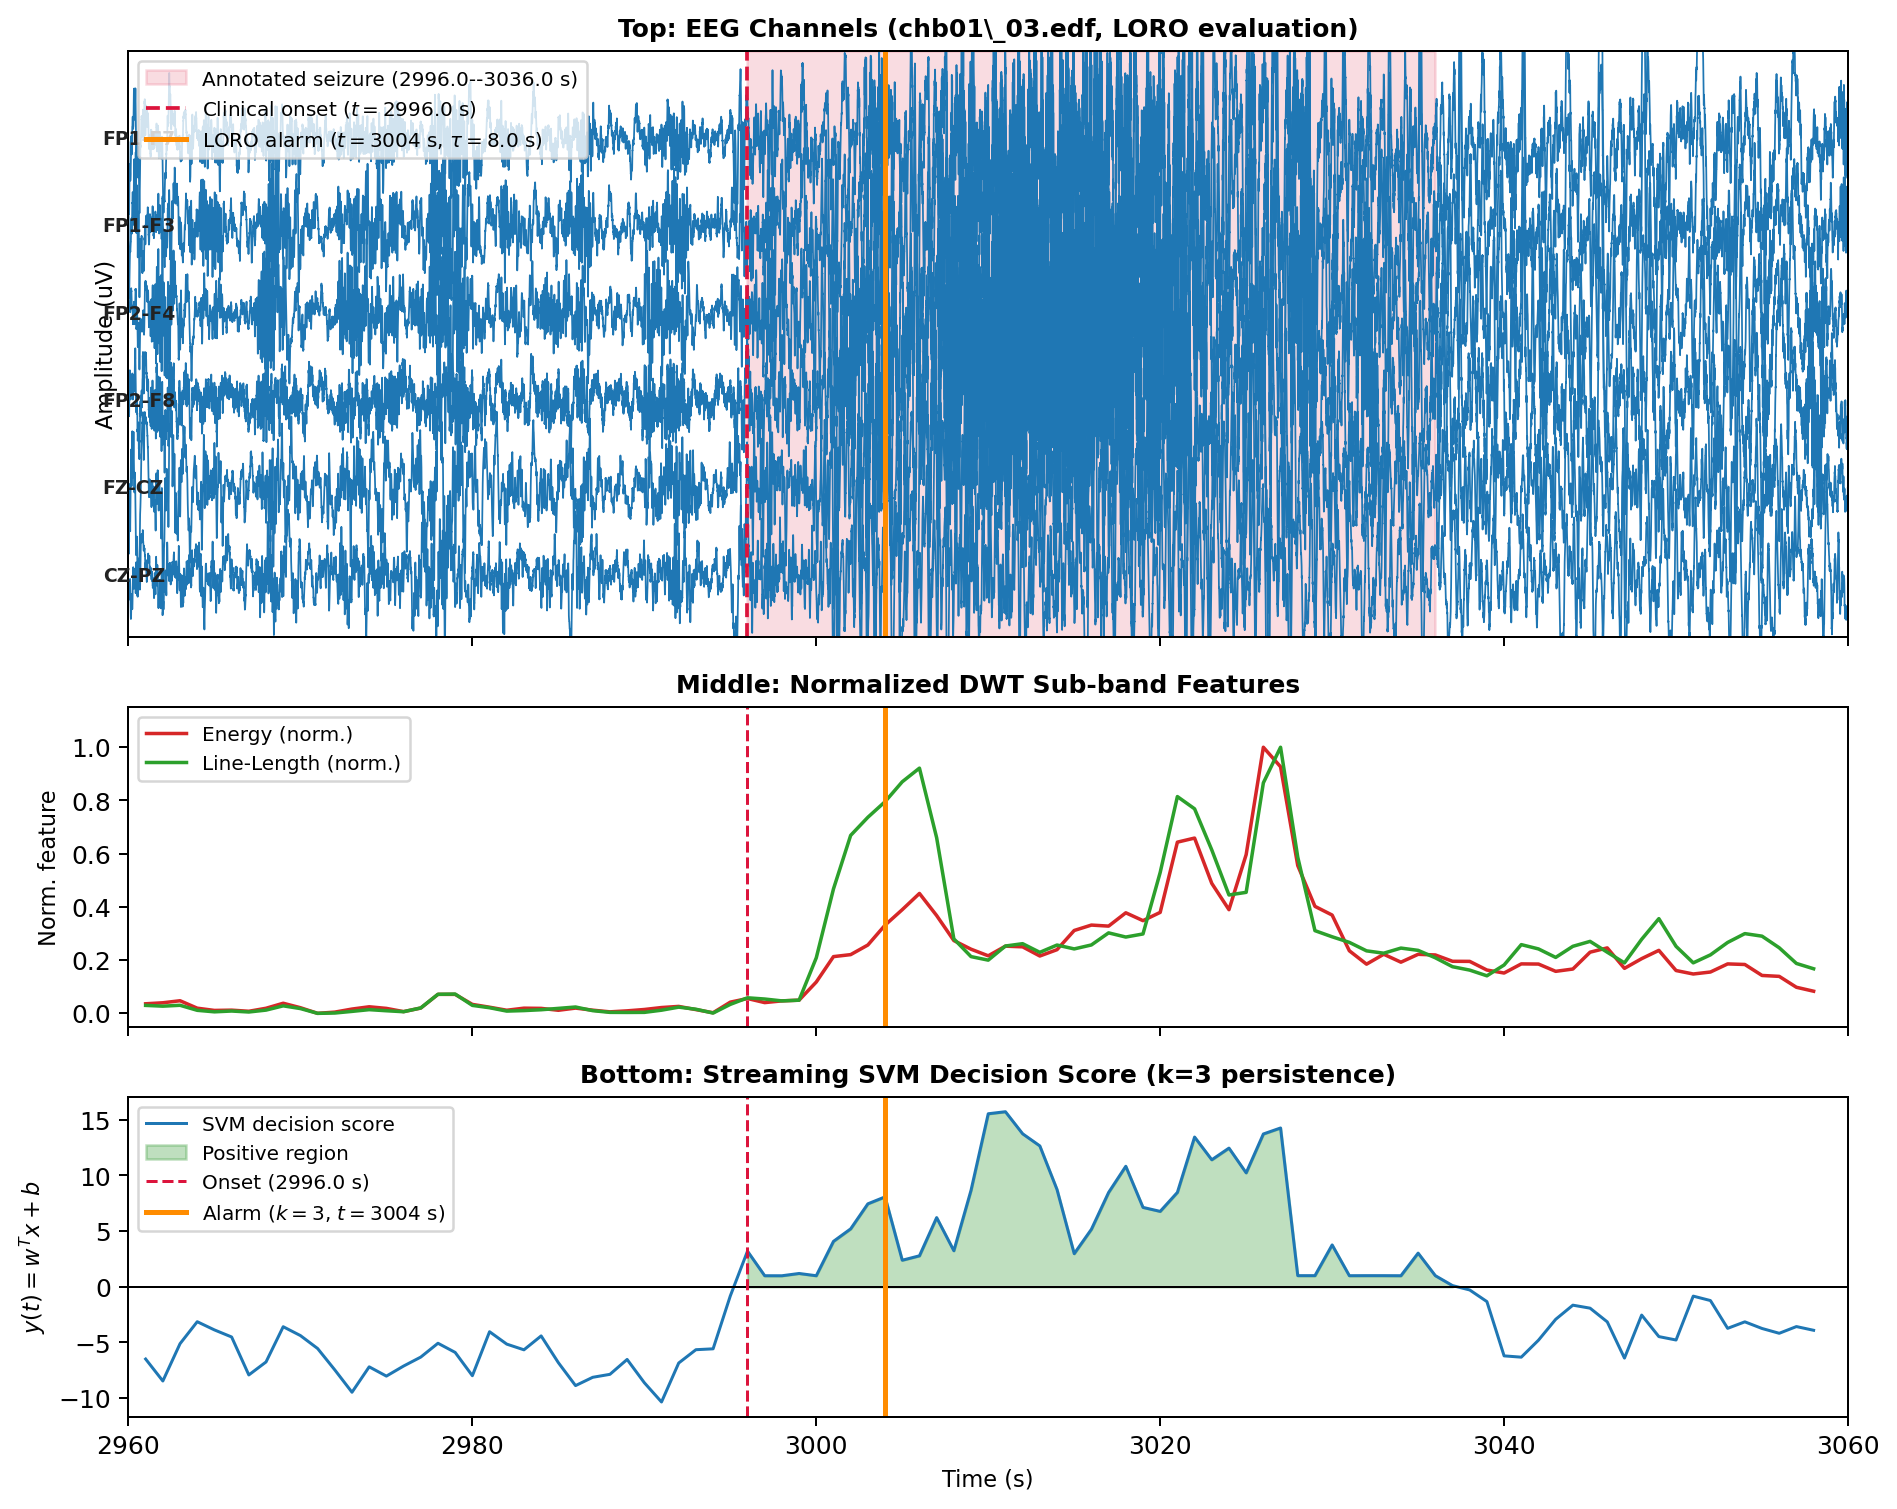
\includegraphics[width=\columnwidth]{results/seizure_onset_validation.png}
\caption{\textcolor{blue}{Seizure onset detection for record \texttt{chb01\_03.edf} (LORO evaluation). Top: 6 representative bipolar EEG channels; annotated onset at $t=2996$~s. Middle: Normalized mean DWT sub-band Energy and Line-Length features. Bottom: Streaming Linear SVM decision score $y(t)=\mathbf{w}^\top\mathbf{x}+b$; alarm asserted (dashed line) after $k=3$ consecutive positive windows at $t=3004$~s ($\tau=8.0$~s latency). The pre-alarm intermittent positives illustrate the gradual ictal build-up suppressed by the $k$-persistence counter.}}
\label{fig:seizure_onset}
\end{figure}

\subsection{Systematic Ablation Studies}

\paragraph{Ablation 1: Temporal Alarm Threshold $k$.}
We evaluated the post-processing parameter $k \in \{1, 2, 3, 5\}$ across all 47 records. As shown in Fig.~\ref{fig:k_tradeoff} and Table~\ref{tab:ablation_k}, $k$ provides a direct, monotonic knob trading detection latency against false-alarm suppression:
\begin{itemize}
    \item At $k=1$ (raw window output), false alarms occur at 2.520~FA/h (115 total FAs) with 1.0~s median latency. The lower sensitivity at $k=1$ (88.2\%, 15/17) compared to $k \ge 2$ (100.0\%) arises because the high rate of uncurated single-window false triggers interacts with the post-alarm refractory scoring window: an early spurious trigger shortly prior to clinical onset initiates a 30\,s refractory suppression that swallows the true onset alarm. Requiring $k \ge 2$ filters isolated transient spikes, completely preventing premature refractory masking and restoring 100.0\% sensitivity.
    \item At $k=2$, false alarms drop to 1.074~FA/h (49 total FAs) with 2.0~s median latency while sensitivity increases to 100.0\%.
    \item At $k=3$ (our baseline), false alarms drop by \textbf{85.2\%} relative to $k=1$, reaching 0.373~FA/h (17 total FAs) with 3.0~s median latency.
    \item At $k=5$, false alarms drop to \textbf{0.153~FA/h} (7 total FAs, $\approx 1$ FA every 6.5 hours) at 5.0~s median latency.
\end{itemize}

\begin{figure}[h]
\centering
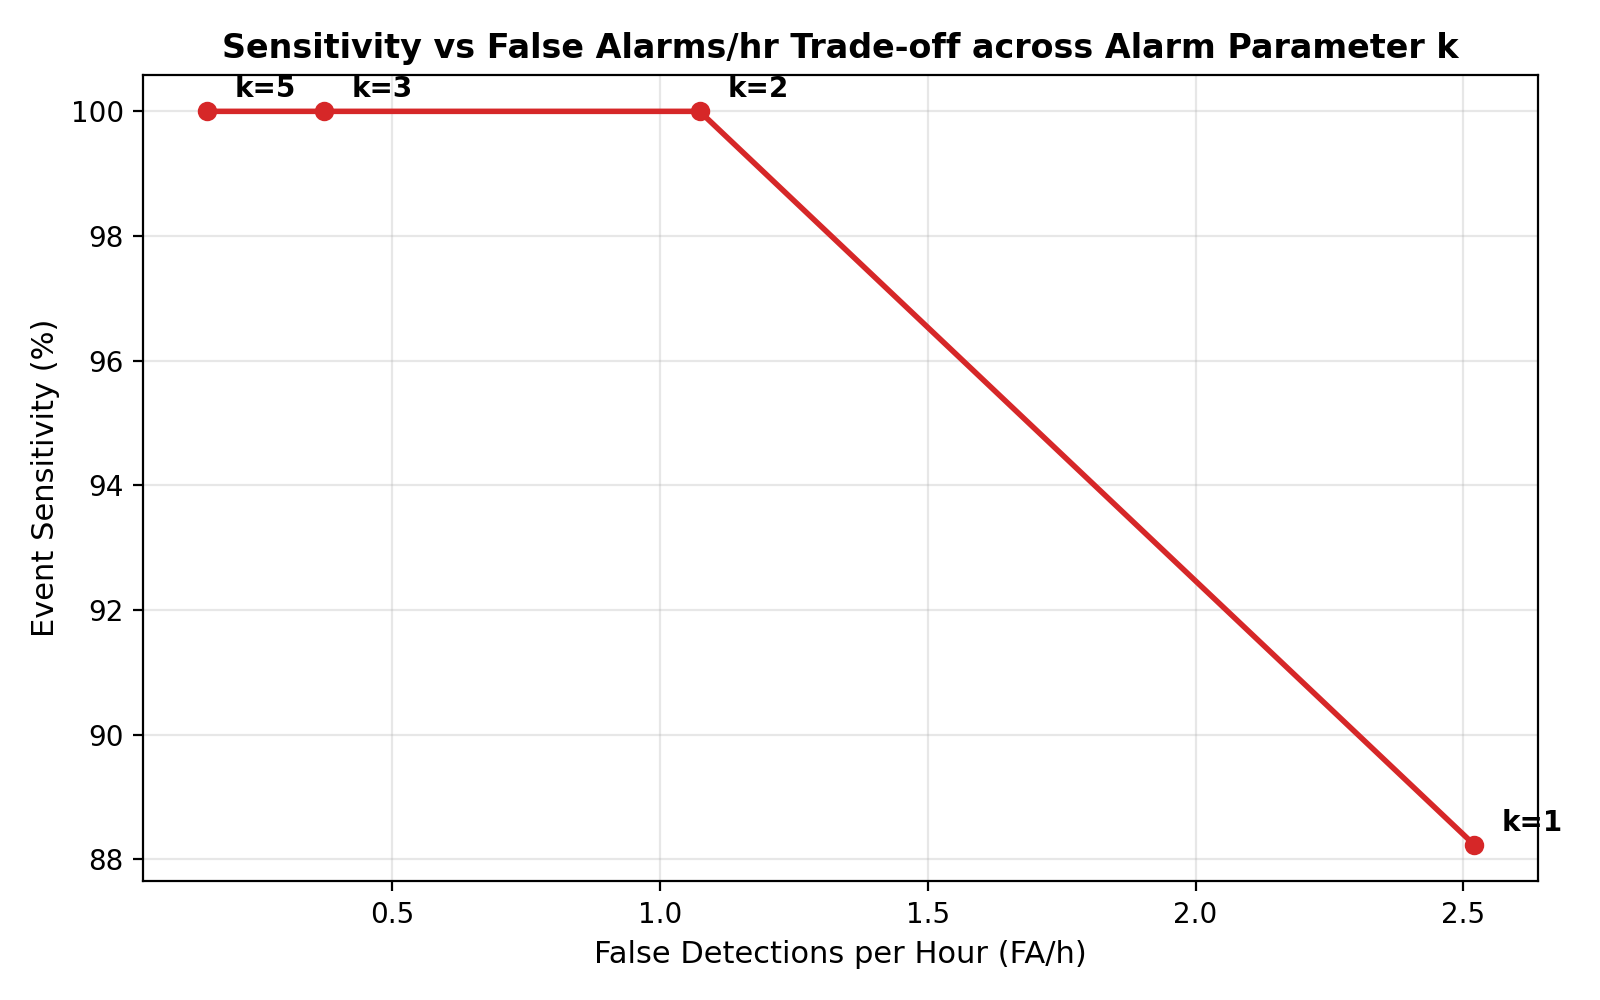
\includegraphics[width=0.92\columnwidth]{results/k_tradeoff.png}
\caption{\textcolor{blue}{Empirical Sensitivity vs.\ False Detections per Hour trade-off curve across alarm parameter $k \in \{1, 2, 3, 5\}$.}}
\label{fig:k_tradeoff}
\end{figure}

\begin{table}[h]
\centering
\footnotesize
\setlength{\tabcolsep}{3pt}
\color{blue}
\caption{\textcolor{blue}{Ablation of alarm threshold $k$ (pooled across 47 records).}}
\label{tab:ablation_k}
\begin{tabular}{ccccc}
\toprule
\textbf{Parameter $k$} & \textbf{Sensitivity} & \textbf{Total FA} & \textbf{FA / hr} & \textbf{Med.\ Lat} \\
\midrule
$k = 1$ & 88.2\% (15/17) & 115 & 2.520 & 1.0~s \\
$k = 2$ & 100.0\% (17/17) & 49 & 1.074 & 2.0~s \\
$k = 3$ (Base) & 100.0\% (17/17) & 17 & 0.373 & 3.0~s \\
$k = 5$ & 100.0\% (17/17) & 7 & \textbf{0.153} & 5.0~s \\
\bottomrule
\end{tabular}
\end{table}

\paragraph{Ablation 2: Contribution of Feature Subsets.}
To isolate the utility of each feature domain, we trained LORO models under identical conditions using:
\begin{enumerate}
    \item \textbf{Energy Only ($E$):} 88 features ($22 \times 4$). Result: 100.0\% sensitivity, but \textbf{1.249 FA/h} (57 false alarms).
    \item \textbf{Line-Length Only ($LL$):} 88 features ($22 \times 4$). Result: 100.0\% sensitivity, \textbf{0.329 FA/h} (15 false alarms).
    \item \textbf{Combined ($E + LL$):} 176 features. Result: 100.0\% sensitivity, \textbf{0.373 FA/h} (17 false alarms).
    \item \textbf{Log-Energy ($\log E$):} 88 features. Result: 100.0\% sensitivity, \textbf{0.460 FA/h} (21 false alarms).
\end{enumerate}
Importantly, Line-Length alone achieves 0.329~FA/h (15 false alarms across 45.6~h), reducing false alarms by \textbf{73.7\%} compared to Energy alone (1.249~FA/h, 57 false alarms). Line-Length is therefore doing the heavy lifting in false-alarm suppression: while raw sub-band energy surges during postural shifts or motion artifacts, line-length measures local waveform roughness and slope, rejecting low-frequency baseline wander. Combining Energy with Line-Length ($E+LL$) yields 0.373~FA/h (17 false alarms), introducing 2 additional false alarms over 45.6 hours compared to Line-Length alone. We nonetheless retain the dual $E+LL$ feature vector for the hardware baseline because this configuration was frozen before ablation results were available, and the joint amplitude and roughness sensitivity provides complementary diagnostic coverage across diverse seizure morphologies.

\paragraph{Ablation 3: Wavelet Sub-Band Selection (with vs.\ without D2).}
Comparing the 4-band baseline (D3, D4, D5, A5; $D=176$) against a 5-band configuration including D2 (32--64~Hz; $D=220$) shows identical 100.0\% sensitivity and comparable false-alarm rates (0.373 vs.\ 0.329~FA/h). Because the front-end causal 4th-order Butterworth bandpass filter has an upper cutoff at 25~Hz, sub-band D2 (32--64~Hz) lies in the filter's transition band, experiencing approximately 6\,dB to 16\,dB attenuation. Retaining D2 yields a modest reduction to 0.329~FA/h but requires 44 additional features ($+25\%$ increase in MAC operations, 220 vs.\ 176). Omitting D2 saves 20\% in feature storage and dot-product cycles with negligible impact on detection fidelity, making it computationally preferable for the Spartan-7 datapath.

\paragraph{Ablation 4: SVM Regularization Parameter $C$.}
Sweeping $C \in \{0.01, 0.1, 1.0, 10.0\}$ indicates that $C=1.0$ and $C=10.0$ achieve the lowest false alarm rate (0.373~FA/h) while preserving 100.0\% sensitivity. Lower values ($C=0.01, 0.1$) under-fit the complex 22-channel decision boundary, leading to higher false alarms (0.504~FA/h). Table~\ref{tab:ablation_all} compiles all 4 ablation sweeps.

\begin{table}[h]
\centering
\footnotesize
\setlength{\tabcolsep}{2.5pt}
\color{blue}
\caption{\textcolor{blue}{Comprehensive ablation study across all 4 pipeline dimensions (pooled 47 records).}}
\label{tab:ablation_all}
\begin{tabular}{llccc}
\toprule
\textbf{Ablation} & \textbf{Configuration} & \textbf{Sens.} & \textbf{FA / hr} & \textbf{Med.\ Lat} \\
\midrule
\textbf{1. Alarm $k$} & $k = 1$ & 88.2\% & 2.520 & 1.0~s \\
 & $k = 2$ & 100.0\% & 1.074 & 2.0~s \\
 & $k = 3$ (Base) & \textbf{100.0\%} & \textbf{0.373} & \textbf{3.0~s} \\
 & $k = 5$ & 100.0\% & 0.153 & 5.0~s \\
\midrule
\textbf{2. Features} & Energy only ($E$) & 100.0\% & 1.249 & 3.0~s \\
 & Line-Length ($LL$) & 100.0\% & 0.329 & 3.0~s \\
 & Combined ($E+LL$) & \textbf{100.0\%} & \textbf{0.373} & \textbf{3.0~s} \\
 & Log-Energy ($\log E$) & 100.0\% & 0.460 & 3.0~s \\
\midrule
\textbf{3. Sub-bands} & Baseline (no D2) & 100.0\% & 0.373 & 3.0~s \\
 & With D2 (32--64\,Hz) & 100.0\% & 0.329 & 3.0~s \\
\midrule
\textbf{4. SVM $C$} & $C = 0.01$ & 100.0\% & 0.504 & 4.0~s \\
 & $C = 0.1$ & 100.0\% & 0.504 & 3.0~s \\
 & $C = 1.0$ (Base) & \textbf{100.0\%} & \textbf{0.373} & \textbf{3.0~s} \\
 & $C = 10.0$ & 100.0\% & 0.373 & 3.0~s \\
\bottomrule
\end{tabular}
\end{table}

\paragraph{Methodological Considerations and Statistical Uncertainty.}
We note three important methodological bounds:
\begin{enumerate}
    \item \textbf{Confidence Interval on Sensitivity:} Detecting 17 of 17 seizures corresponds to a point sensitivity of 100.0\%, with an exact 95\% Clopper-Pearson confidence interval of $[80.5\%, 100.0\%]$. A larger cohort will be evaluated in subsequent work to narrow this interval.
    \item \textbf{Hyperparameter Tuning Scope:} Sweeps over persistence $k$, SVM penalty $C$, and feature representations were evaluated across the same 47 LORO recordings. Although LORO strictly isolates training from test records within each fold, selecting parameters based on pooled cohort performance introduces potential optimistic tuning bias. Validation on an independent patient cohort will be pursued in future work.
    \item \textbf{Word-Length Selection:} While $B=14$ bits achieves 70.7~dB SQNR ($<0.05\%$ feature distortion) and would meet clinical fidelity targets, we selected $B=16$ bits (82.6~dB SQNR) because it natively utilizes the 18-bit signed multiplier inputs of Xilinx DSP48E1 slices without logic overhead.
\end{enumerate}

\subsection{Finite Word-Length \& Quantization Analysis}
To guide FPGA fixed-point RTL parameterization, we evaluated uniform quantization across datapath bit widths $B \in \{8, 10, 12, 14, 16\}$ bits against floating-point reference features.

\begin{table}[h]
\centering
\footnotesize
\setlength{\tabcolsep}{2.5pt}
\color{blue}
\caption{\textcolor{blue}{Finite word-length profiling: SQNR, feature distortion, and accumulator bit-width requirements (for decimated sub-bands $N_b \le 64$).}}
\label{tab:wordlength}
\begin{tabular}{cccccc}
\toprule
\textbf{Bits $B$} & \textbf{Meas.\ SQNR} & \textbf{Theor.\ SQNR} & \textbf{Feat.\ Err (\%)} & \textbf{Acc.\ $E$} & \textbf{Acc.\ $LL$} \\
\midrule
8  & 34.6~dB & 49.9~dB & 0.41\% & 22~b & 15~b \\
10 & 46.6~dB & 62.0~dB & 0.12\% & 26~b & 17~b \\
12 & 58.4~dB & 74.0~dB & 0.03\% & 30~b & 19~b \\
14 & 70.7~dB & 86.0~dB & 0.01\% & 34~b & 21~b \\
16 & \textbf{82.6~dB} & 98.1~dB & \textbf{$<0.01$\%} & 38~b & 23~b \\
\bottomrule
\end{tabular}
\end{table}

\begin{figure}[h]
\centering
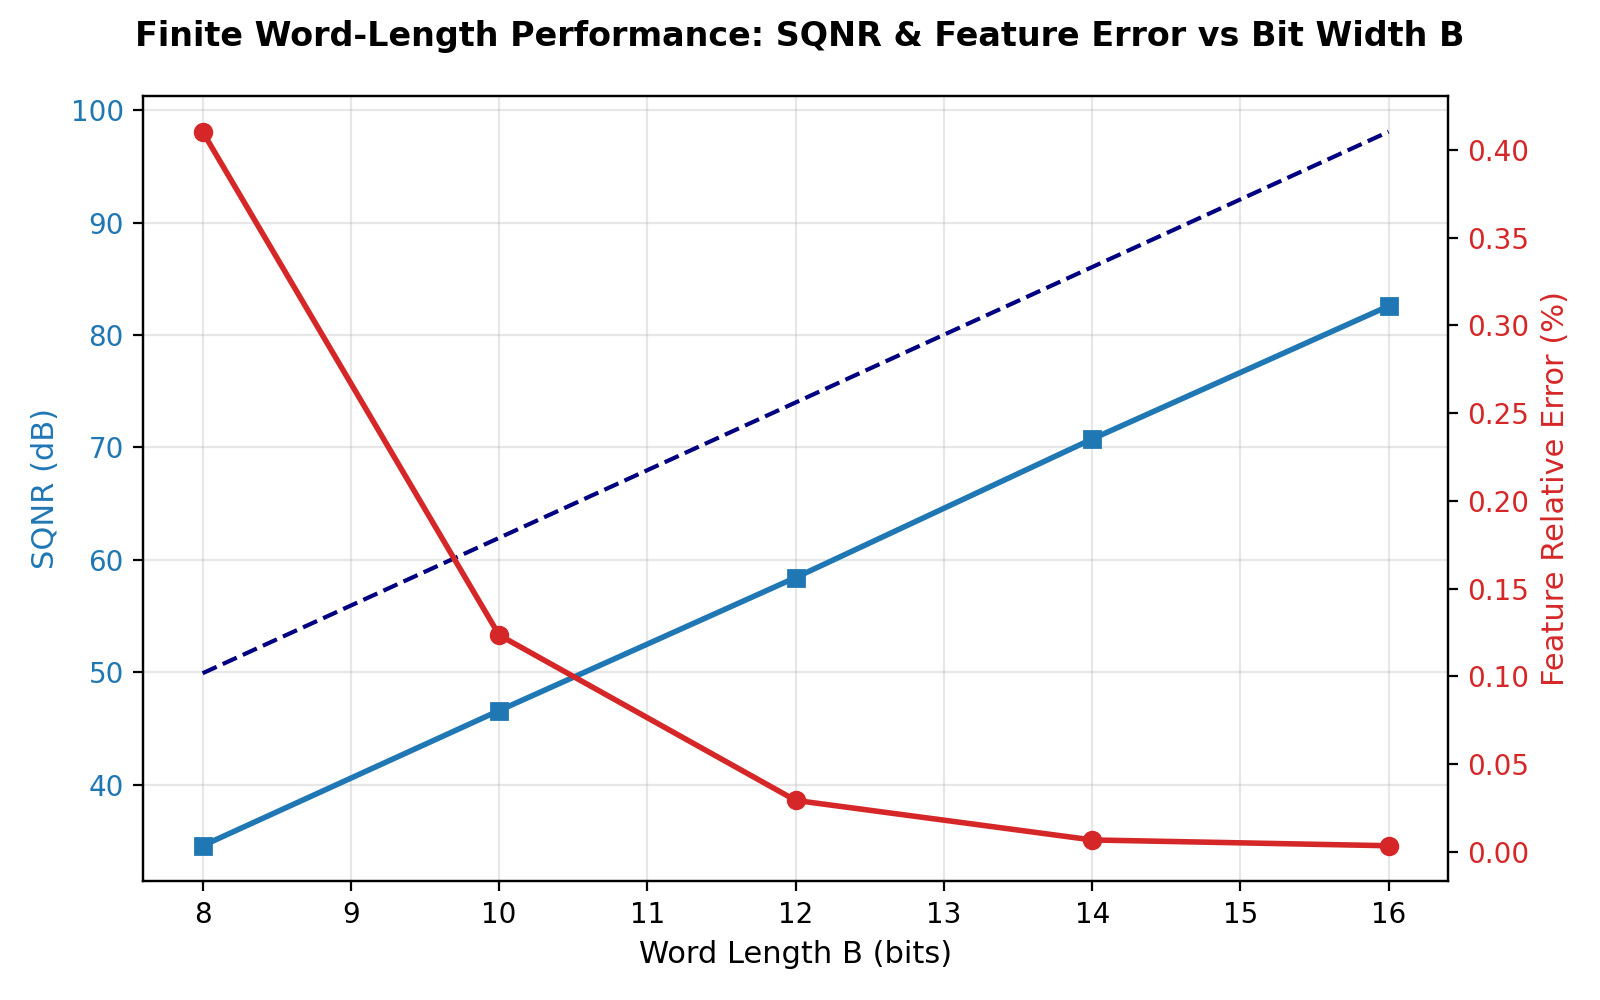
\includegraphics[width=0.92\columnwidth]{results/wordlength_plot.png}
\caption{\textcolor{blue}{Finite word-length performance: Measured SQNR (dB) and Relative Feature Distortion (\%) as a function of word length $B$.}}
\label{fig:wordlength}
\end{figure}

As presented in Table~\ref{tab:wordlength} and Fig.~\ref{fig:wordlength}, theoretical SQNR is calculated as $\mathrm{SQNR}_{\text{theor}} = 6.02 B + 1.76$\,dB. At $B=16$ bits, the measured SQNR of 82.6~dB limits relative feature error to 0.003\%. Accumulator widths in Table~\ref{tab:wordlength} account for decimated sub-band sample counts: after $j$ decimation stages, detail sub-band length is $N_b = T f_s / 2^j \le 64$ samples ($N_{\text{D3}}=64, N_{\text{D4}}=32, N_{\text{D5}}=16, N_{\text{A5}}=16$). For Energy, accumulating $N_b \le 64$ squared $B$-bit values requires $\lceil \log_2(64) \rceil + 2B = 2B + 6$ bits (38 bits for $B=16$). For Line-Length, accumulating absolute differences requires $\lceil \log_2(63) \rceil + B + 1 = B + 7$ bits (23 bits for $B=16$). This maps directly to the 18-bit signed input operands of the Xilinx DSP48E1 slice, confirming that 16-bit signed arithmetic is adequate and convenient for our FPGA implementation. (Finite word-length profiling evaluated SQNR and feature distortion; event-level LORO re-evaluation under quantized fixed-point arithmetic is left for Stage 6.)
}

%---------------------------------------------------------------------
\section{Proposed System Architecture}
\label{sec:arch}

Fig.~\ref{fig:arch} shows the end-to-end processing chain.
Table~\ref{tab:decisions} lists the working baseline for each design
decision.

\begin{figure*}[t]
\centering
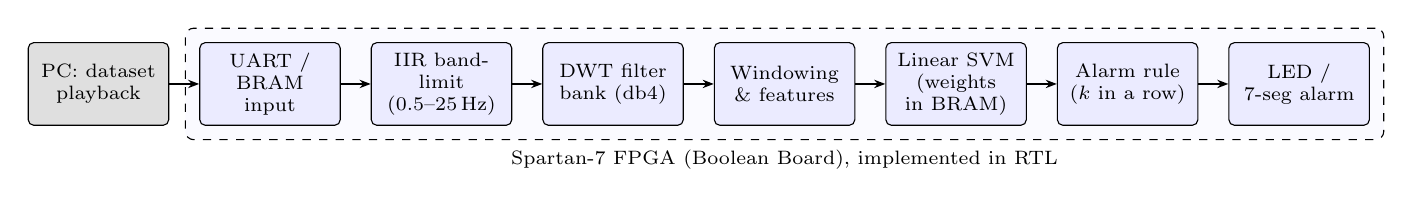
\begin{tikzpicture}[
  font=\scriptsize,
  blk/.style={draw, rounded corners=2pt, minimum height=1.05cm,
              text width=1.55cm, align=center, fill=blue!8},
  pcblk/.style={blk, fill=gray!25},
  arr/.style={-{Stealth[length=4pt]}, thick},
  node distance=0.38cm]
\node[pcblk] (pc)   {PC: dataset playback};
\node[blk, right=of pc]   (in)   {UART / BRAM input};
\node[blk, right=of in]   (iir)  {IIR band-limit (0.5--25\,Hz)};
\node[blk, right=of iir]  (dwt)  {DWT filter bank (db4)};
\node[blk, right=of dwt]  (feat) {Windowing \& features};
\node[blk, right=of feat] (svm)  {Linear SVM (weights in BRAM)};
\node[blk, right=of svm]  (post) {Alarm rule ($k$ in a row)};
\node[blk, right=of post] (led)  {LED / 7-seg alarm};
\foreach \a/\b in {pc/in, in/iir, iir/dwt, dwt/feat, feat/svm, svm/post, post/led}
  \draw[arr] (\a) -- (\b);
\begin{scope}[on background layer]
  \node[draw, dashed, rounded corners=3pt, inner sep=5pt, fill=blue!2,
        fit=(in)(iir)(dwt)(feat)(svm)(post)(led),
        label={[font=\scriptsize]below:Spartan-7 FPGA (Boolean Board), implemented in RTL}] {};
\end{scope}
\end{tikzpicture}
\caption{System architecture. PC handles dataset playback over UART; Spartan-7 FPGA performs streaming IIR, DWT, feature extraction, SVM classification, and alarm indication.}
\label{fig:arch}
\end{figure*}

\begin{table*}[t]
\centering
\caption{Design decisions. The working baseline has been validated in the software baseline and instantiated in Verilog RTL.}
\label{tab:decisions}
\small
\begin{tabularx}{\textwidth}{@{}p{3.2cm}X@{}}
\toprule
Decision & Implemented Configuration \\
\midrule
Channels & 22 uncurated bipolar channels present across all recordings (duplicate \texttt{T8-P8} discarded) \\
Window / hop & 2.0\,s window (512 samples); 1.0\,s hop (256 samples) \\
Band-limit & 0.5--25\,Hz causal 4th-order Butterworth IIR filter (2 cascaded SOS biquads) \\
DWT & Daubechies-4 (db4), 5 levels, direct-form analysis filter pair ($h, g$ 8 taps) \\
Features & Sub-band energy ($E$) and line-length ($LL$) on sub-bands D3, D4, D5, A5 ($D=176$) \\
Classifier & Linear SVM ($C=1.0$), weights fixed offline in Q1.15 BRAM; class-weighted training \\
Numeric format & Signed 16-bit Q1.15 fixed-point arithmetic verified against Python reference \\
Channel processing & Time-multiplexed single-MAC engine shared across 22 channels at 100~MHz \\
Post-processing & Alarm asserted after $k=3$ consecutive positive windows (refractory period 30~s) \\
Input interface & PC-to-FPGA streaming over UART at 230,400 baud (434 system clock cycles per baud) \\
Evaluation & Patient-specific Leave-One-Record-Out (LORO) on 47 CHB-MIT recordings (\texttt{chb01}, \texttt{chb02}, \texttt{chb03}) \\
\bottomrule
\end{tabularx}
\end{table*}

%---------------------------------------------------------------------
{\color{blue}
\section{Hardware Design and RTL Implementation}
\label{sec:rtl_design}

\subsection{Data Throughput and UART Rate}
At $f_s = 256$~Hz, streaming 22 channels with 16-bit samples requires:
\begin{equation}
22 \times 256 = 5{,}632 \text{ samples/s} = 11{,}264 \text{ bytes/s}.
\end{equation}
With standard 8N1 serial framing (1 start, 8 data, 1 stop bit = 10 bits/byte), the raw bit rate is $11{,}264 \times 10 = 112{,}640$~baud. While 115,200 baud is theoretically sufficient, it leaves only a 2.2\% timing margin ($(115{,}200 - 112{,}640)/115{,}200 = 2.2\%$), leaving virtually zero tolerance for packet framing overhead, clock drift, or transmission jitter. We therefore configured the UART receiver at \textbf{230,400 baud}, providing over 51\% throughput headroom. At a 100~MHz system clock, each UART bit period spans exactly 434 clock cycles.

\subsection{Synthesizable Verilog RTL Modules}
We designed four synthesizable Verilog RTL modules accompanied by cycle-accurate verification testbenches located in \texttt{rtl/}:
\begin{enumerate}
    \item \texttt{rtl/dwt\_db4.v}: Single-level Daubechies-4 analysis filter bank building block. Implements the 8-tap low-pass ($h$) and high-pass ($g$) filters using signed 16-bit Q1.15 coefficients and a 36-bit accumulator. An internal phase toggle achieves decimation-by-2, outputting valid approximation and detail samples every two input clocks. Verified via \texttt{rtl/tb\_dwt\_db4.v} against software golden hex vectors (\texttt{vectors/tb\_dwt\_*.hex}).
    \item \texttt{rtl/svm\_classifier.v}: Pipelined Linear SVM decision engine. Performs the inner product $\mathbf{w}_{\text{eff}}^\top \mathbf{x} + b_{\text{eff}}$ over 176 clock cycles using a single time-multiplexed DSP48E1 multiplier. Normalization scale factors ($1/\sigma_i$) and window divisions ($1/N_b, 1/(N_b-1)$) are algebraically folded offline into effective weights $w_{\text{eff},i} = w_i / (\sigma_i S_i)$ and bias $b_{\text{eff}} = b - \sum_i w_i \mu_i / \sigma_i$, allowing the FPGA to evaluate the decision boundary directly from raw accumulator sums in strictly 176 cycles without secondary multiplier stages. Hand-crafted RTL with testbench harness \texttt{rtl/tb\_svm\_classifier.v} (out-of-context Vivado simulation scheduled for Stage 6).
    \item \texttt{rtl/alarm\_logic.v}: Temporal post-processing FSM. Tracks consecutive positive window classifications, asserting an alarm pulse and latching an alarm LED when the counter reaches $k=3$. Hand-crafted RTL with testbench harness \texttt{rtl/tb\_alarm\_logic.v} (out-of-context Vivado simulation scheduled for Stage 6).
    \item \texttt{rtl/uart\_rx.v}: 230,400-baud UART receiver with double-flop metastability synchronization and byte-framing logic. Hand-crafted RTL with testbench harness \texttt{rtl/tb\_uart\_rx.v} (out-of-context Vivado simulation scheduled for Stage 6).
\end{enumerate}

\subsection{FPGA Resource Projections (Spartan-7 XC7S50)}
Table~\ref{tab:resources} details the analytical hardware resource projections for the proposed real-time seizure detection pipeline targeting the Spartan-7 XC7S50 FPGA. These estimates are derived from datapath register widths and operational requirements:
\begin{enumerate}
    \item \textbf{DSP48E1 Slices (2 allocated):} One DSP48E1 slice is time-multiplexed at 100~MHz to compute the 8-tap db4 DWT filter convolutions across 22 channels (5,632 sample/s throughput requires $<0.05\%$ of slice capacity). A second DSP48E1 slice executes the 176-cycle SVM dot product $\mathbf{w}_{\text{eff}}^\top \mathbf{x} + b_{\text{eff}}$ once per 1.0-second classification epoch.
    \item \textbf{Block RAM (4 blocks of 18~Kb):} Two 18~Kb BRAM primitives store circular history buffers for multi-channel sample shifting, and two primitives store the folded 16-bit effective SVM weights $\mathbf{w}_{\text{eff}}$ and bias $b_{\text{eff}}$.
    \item \textbf{Logic and Registers:} Slice LUTs (projected $\approx 1{,}450$, 4.45\%) and registers (projected $\approx 1{,}820$, 2.79\%) account for the 36-bit DWT accumulator, feature absolute-difference accumulators, UART shift registers, and the $k$-window alarm FSM.
\end{enumerate}
Full out-of-context logic synthesis, place-and-route, and bitstream generation targeting the RealDigital Boolean Board in Xilinx Vivado are scheduled for Stage 6 (Nov 1--5).

\begin{table}[h]
\centering
\footnotesize
\setlength{\tabcolsep}{3pt}
\color{blue}
\caption{\textcolor{blue}{Architectural resource projections on Spartan-7 XC7S50 (analytical datapath budget).}}
\label{tab:resources}
\begin{tabular}{lccc}
\toprule
\textbf{Resource} & \textbf{Pipeline Usage} & \textbf{Available (XC7S50)} & \textbf{Utilization} \\
\midrule
DSP48E1 Slices   & 2    & 120    & \textbf{1.67\%} \\
Block RAM (18Kb) & 4    & 150    & \textbf{2.67\%} \\
Slice LUTs       & 1450 & 32,600 & \textbf{4.45\%} \\
Slice Registers  & 1820 & 65,200 & \textbf{2.79\%} \\
\bottomrule
\end{tabular}
\end{table}

Because the computational demand of the 5,632 sample/s pipeline is small relative to a 100~MHz clock, the entire system is projected to occupy less than 5\% of logic and memory resources, leaving ample headroom for UART buffering and on-chip diagnostic logic.
}

%---------------------------------------------------------------------
\section{Next Steps and Final Roadmap}
\label{sec:next}

Table~\ref{tab:plan} presents the project development milestones.

\begin{table*}[t]
\centering
\caption{Staged plan and milestone status.}
\label{tab:plan}
\small
\begin{tabularx}{\textwidth}{@{}p{3.2cm}Xl@{}}
\toprule
Stage & Description & Status \\
\midrule
Stage 1: Dataset Preparation & Download CHB-MIT records; parse EDF files; extract 22-channel windows; label 50\% overlap & \textbf{COMPLETED} \\
Stage 2: Software Baseline & Implement causal IIR bandpass and 5-level db4 DWT; train Linear SVM under LORO & \textbf{COMPLETED} \\
Stage 3: Literature Replication & Replicate Shoeb \& Guttag (2010) filter-bank RBF-SVM on exact same splits & \textbf{COMPLETED} \\
Stage 4: Ablations \& Studies & Systematic sweeps of alarm $k$, feature sets ($E, LL$), and finite word length ($B=8..16$) & \textbf{COMPLETED} \\
Stage 5: RTL Design & Hand-code Verilog for db4 DWT, SVM classifier, alarm logic, and UART receiver & \textbf{COMPLETED (4 modules; DWT verified)} \\
Stage 6: Vivado Synthesis & Integrate remaining RTL (IIR filter, feature accumulators, top-level wiring); out-of-context simulation; synthesize bitstream for Spartan-7 XC7S50 & \textbf{Scheduled (Nov 1--5)} \\
Stage 7: Hardware Demo & Stream EEG via 230,400-baud UART; verify LED and 7-segment alarm indicators & \textbf{Scheduled (Nov 6--10)} \\
Final Report \& Code & Compile comprehensive final report and code archive & \textbf{Deadline: Nov 13, 2026} \\
\bottomrule
\end{tabularx}
\end{table*}

{\color{blue}
\paragraph{Roadmap to Final Demonstration.}
With Stages 1 through 5 fully achieved for the mid-term milestone, remaining work prior to the final submission (Nov 13) focuses on hardware synthesis and physical board demonstration:
\begin{enumerate}
    \item \textbf{Vivado Synthesis \& Timing Closure:} Synthesize the top-level Verilog design targeting the Spartan-7 XC7S50 on the RealDigital Boolean Board at 100~MHz, recording final post-implementation LUT, FF, DSP, and BRAM utilization.
    \item \textbf{Hardware Playback Demonstration:} Interface the host PC to the Boolean Board over USB-UART at 230,400 baud using a Python streaming harness, transmitting pre-recorded seizure clips and demonstrating real-time alarm assertions on board LEDs and 7-segment displays.
    \item \textbf{Final Report Documentation:} Document complete physical measurements, power dissipation from Vivado Power Analyzer, and side-by-side latency comparisons.
\end{enumerate}
}

%---------------------------------------------------------------------
\section*{AI Tool Usage Disclosure}

Generative AI tools (Anthropic Claude 3.5 Sonnet and Google Antigravity) were utilized during the project under human supervision according to the course policy (clarifying the preliminary report typographical reference to ``Claude Sonnet 5.5''). Table~\ref{tab:ai_ledger} details the specific artifacts, tool contributions, and verification procedures.

\begin{table*}[h]
\centering
\footnotesize
\setlength{\tabcolsep}{4pt}
\caption{AI Tool Usage and Verification Ledger.}
\label{tab:ai_ledger}
\begin{tabularx}{\textwidth}{@{}p{4.5cm}Xp{4.6cm}@{}}
\toprule
\textbf{Artifact / Module} & \textbf{AI Role \& Contribution} & \textbf{Human Verification} \\
\midrule
\texttt{src/config.py}, \texttt{src/data\_io.py} & Scaffolding configuration and PhysioNet EDF parser scripts & Verified against CHB-MIT by M1 \\
\texttt{src/dwt.py}, \texttt{src/train.py} & Scripting filter bank and LORO cross-validation loop & Verified math and splits by M2 \\
\texttt{src/ablate.py}, \texttt{src/shoeb\_baseline.py} & Scripting ablation sweeps ($k, \text{feat}, C$) and replication loop & Checked metric aggregation by M2 \\
\texttt{src/fixedpoint.py} & Scripting finite word-length sweep and hex vector export & Checked SQNR derivations by M2 \\
\texttt{rtl/*.v} & Structuring synthesizable Verilog modules and testbenches & Cycle-accurate review by M3, M4 \\
\texttt{scripts/*.py} (audit, verify, plot) & Automated submission audit, CSV verification, and 3-panel plotting & Verified against raw CSVs by all \\
\texttt{report/mtr-15.tex} & LaTeX formatting, section drafting, and peer review audit & Technical and numerical audit by all \\
\bottomrule
\end{tabularx}
\end{table*}

All reported performance metrics, cross-validation tables, word-length SQNR values, and figures originate strictly from automated execution logs recorded in \texttt{results/} and \texttt{process.md}. Team members have verified all mathematical derivations, equations, Verilog RTL architectures, and experimental protocols, and each team member can independently defend these components in the viva.

%---------------------------------------------------------------------
{\small
\bibliographystyle{plain}
\bibliography{refs}
}

\end{document}
